\subsection{Android}

\par
Android es un sistema operativo basado en el núcleo Linux. Fue diseñado principalmente para dispositivos móviles con pantalla táctil, como teléfonos inteligentes, tablets o tabléfonos; y también para relojes inteligentes, televisores y automóviles. Inicialmente fue desarrollado por Android Inc. la cual fue fundado en 2003 por Andy Rubin, Rich Miner, Nick Sears y Chris White con el objetivo de desarrollar \textquotedblleft dispositivos móviles que están al corriente de la ubicación y preferencias del usuario \textquotedblright\cite{android-wiki}. En un principio la intención era desarrollar un sistema operativo avanzado para cámaras digitales, pero más tarde se cambió el foco al determinar que el mercado de las cámaras digitales no era lo suficientemente grande. Se redirigirían los esfuerzos a crear un sistema que pudiera competir con Symbian y Windows Mobile\cite{android-xataka}. La versión básica de Android es conocida como Android Open Source Project (AOSP)\cite{android-wiki}. A continuación, una imagen de la evolución del logo de Android. 

\begin{figure}[H]
	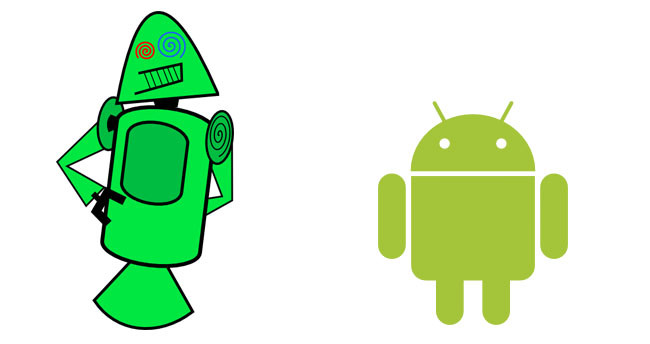
\includegraphics[width=\textwidth]{android1.jpg}
	\caption{Diseño preliminar para el logo de Android (Izquierda) y el logo oficial (Derecha)}
\end{figure}

\par \noindent
A partir del año 2011 Google ha ido actualizando la versión de Android, todos los años. Hoy en día la última versión de Android es \textquotedblleft Android 8.0 Oreo \textquotedblright. Sin embargo, la versión de Android con más dispositivo o smartphones, en uso actualmente, es Android 5.0 Lollipop, la cual será presentada a continuación.

\subsubsection{Android 5.0 Lollipop} 

\par 
Android Lollipop es una versión del sistema operativo para dispositivos móviles Android. Fue dada a conocer el 25 de junio de 2014 durante el Google I/O 2014 como Android L, Google I/O es una conferencia anual presentada por Google en sus oficinas en Mountain View, California.
Los cambios más prominentes en Lollipop incluyen una interfaz de usuario rediseñada construida sobre un diseño de lenguaje responsivo denominado como \textquotedblleft Material design\textquotedblright, así como mejoras en el sistema de notificaciones que permiten que este sea accedido desde la pantalla de bloqueo, y mostrado junto con otras aplicaciones como banners en la parte superior de la pantalla. También se realizaron cambios internos para mejorar y optimizar el rendimiento de consumo de batería en smartphones\cite{lollipop}.

\begin{figure}[H]
	\centering
	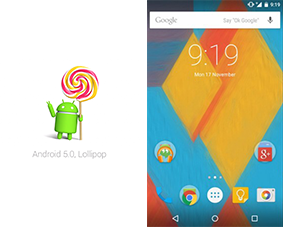
\includegraphics[width=7cm, height=6cm]{android2.png}
	\caption{Logo oficial (Izquierda) e Interfaz móvil (Derecha) de Android 5.0 Lollipop}
\end{figure}

\par \noindent
Ahora veremos las tecnologías que se aplicaran en el área de la electrónica.